\chapter{Game Rules}
\label{game_rules}

 Understanding a game’s rules is the first step toward analyzing it. They provide the foundation for studying the game’s complexity, developing strategies, and designing AI agents capable of playing at a high level.

In this chapter, we present the rules of \textbf{Tricolor} as described in the original patent, with one exception. In theory, a game of Tricolor can continue indefinitely if the players choose to do so, since the original rules do not include a condition that forces the game to end. This absence is problematic when analyzing the game through thousands of simulations,\footnote{Some games could otherwise last for an extremely large number of turns.} as it may lead to excessively long games. To address this issue, we introduce an additional rule, presented at the end of this chapter, that guarantees termination.

\section{Number of players}

In the original patent for Tricolor it's specified that the number of players can be 2 or 3, but in this paper I will only consider the 2 players version.

\section{Board and Pieces setup}

The board uses a hexagonal tiling containing 3 different colors. Each player starts with 18 pieces on his side of the board as shown in Figure~\ref{fig:board_setup}. Player 1 has the white pieces and player 2 the black pieces.

\begin{figure}[h]
    \centering
    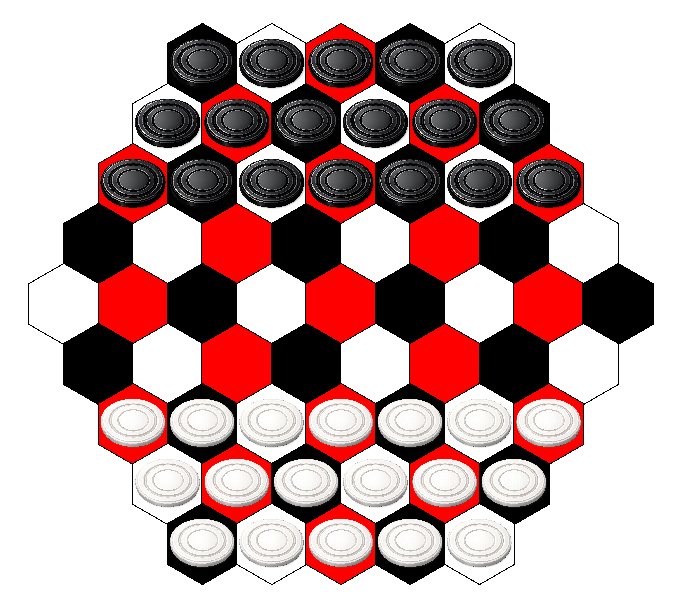
\includegraphics[scale=0.5]{game_rules/images/board_setup.png}
    \caption{Initial board setup}
    \label{fig:board_setup}
\end{figure}

\section{Gameplay and Rules}
\label{sec:rules}

Each player takes his turn to make one move. By convention, player 1 is always first to move when the game starts. A move consists in selecting one \textbf{stack} of pieces \textbf{controlled} by the player making the move and \textbf{move} any number of pieces \footnote{at least 1} to an \textbf{available} tile.
\\

\textbf{Definitions}:
\begin{itemize}
    \item A \textbf{stack} of pieces is a literal stack that can contain multiple pieces, both white and black. For example, at the start of the game, each player has 18 stacks containing only 1 friendly piece.
    \item A stack is said to be \textbf{controlled} by player 1 (resp. player 2) if the color of the piece on top is white (resp. black e.g. Figure~\ref{fig:stack_example}).
    \begin{figure}[h]
        \centering
        
\includegraphics[scale=0.5]{game_rules/images/stack_example.png}
        \caption{Example of a stack controlled by black}
        \label{fig:stack_example}
    \end{figure}
    \item \textbf{Moving} $x$ pieces from a tile to another means removing the first $x$ pieces from the initial tile, from top to bottom, and placing them on the destination tile.
    \item When moving a stack of pieces, that stack has a so called \textbf{power}. The power of a stack isn't influenced by the number of the opponent's pieces. Therefore,  the \textbf{power} of a stack containing $x$ friendly pieces is the following:
    \[ min(3, x) * color \], where $color$ is a value depending on the color of the initial tile and is as follows:
    \begin{itemize}
        \item \textbf{white} = 1
        \item \textbf{black} = 2
        \item \textbf{red} = 3
    \end{itemize}
    As an example, consider Figure~\ref{fig:stack_2_time_3} and Figure~\ref{fig:stack_3_times_1}.
    Note that the concept of \textbf{power} is also applied to the \textit{defending} stack, which is the stack of pieces controlled by the opponent on the destination tile. The formula is the same as for the \textit{attacking power} of a stack and it takes into account all the opponent pieces found on that tile.
\end{itemize}

\begin{figure}[h]
    \centering
    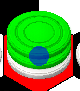
\includegraphics[scale=0.5]{game_rules/images/stack_power_2_times_3.png}
    \caption{Example of an attacking stack (white) with power = $2$ (from 2 selected pieces) * $3$ (color red) = 6}
    \label{fig:stack_2_time_3}
\end{figure}

\begin{figure}[h]
    \centering
    
\includegraphics[scale=0.5]{game_rules/images/stack_3_times_1.png}
    \caption{Example of an attacking stack with power = $3$ (from 3 selected friendly pieces) * $1$ (color white) = 3}
    \label{fig:stack_3_times_1}
\end{figure}

\subsection{How movement works}
\label{sec:rules_movement}

The number of friendly pieces the current player decides to move defines how many tiles he can travel, but it's at most 3 \footnote{e.g. if the player moves 7 friendly pieces the maximal distance he can travel is 3}. Therefore, the number of selected pieces belonging to the opponent doesn't influence the distance allowed to travel. When moving pieces from a tile to another, all the tiles in between must be empty \footnote{If not, you can't make that move}.

A move can be made in the directions shown by the Figure~\ref{fig:move_directions}:

\begin{figure}[h]
    \centering
    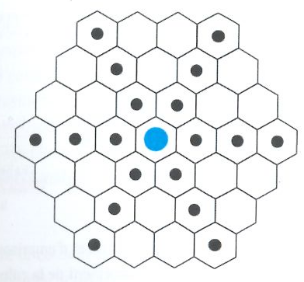
\includegraphics[scale=0.5]{game_rules/images/move_directions.png}
    \caption{All six directions a stack can move in.}
    \label{fig:move_directions}
\end{figure}

\subsection{How the destination tile influences pieces movement}

When moving $x$ pieces from a tile to another, there are 3 possible scenarios:

\begin{enumerate}
    \item The destination tile is empty: in this case, there are no restrictions or exceptions regarding the move.
    \item The destination tile is controlled by you: in this case, as in case 1, there are no restrictions or exceptions regarding the move. The friendly pieces you moved will be stacked on top of the friendly pieces on the destination tile. The opponent pieces you moved will be stacked on top of the opponent pieces on the destination tile, but \textbf{under} your pieces \footnote{You can see this as a reordering of the pieces on the destination tile where all your pieces are on top and the opponent's at the bottom}. As an example, consider Figure~\ref{fig:scenario_2_before} and Figure~\ref{fig:scenario_2_after}
    \begin{figure}[h]
        \centering
        
\includegraphics[scale=0.5]{game_rules/images/scenario_2_before.png}
        \caption{Initial position}
        \label{fig:scenario_2_before}
    \end{figure}
    \begin{figure}[h]
        \centering
        
\includegraphics[scale=0.5]{game_rules/images/scenario_2_after.png}
        \caption{Position after moving to friendly tile (all white pieces are stacked on top and all black pieces are stacked on the bottom)}
        \label{fig:scenario_2_after}
    \end{figure}
    \item The destination tile is controlled by your opponent: in this case, there are again 3 scenarios:
    \begin{enumerate}
        \item The \textbf{power} of the attacking stack is strictly higher than the \textbf{double} of the power of the defending stack: in this case, all the opponent's pieces on the destination tile are completely removed from the game. This move is called a \textbf{capture}. Note, however, that the opponent's pieces belonging to the attacker's stack still remain in the game. As an example, consider Figure~\ref{fig:capture_before} and Figure~\ref{fig:capture_after}.
        \begin{figure}[h]
            \centering
            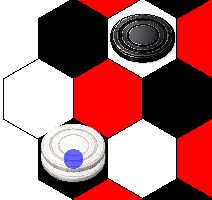
\includegraphics[scale=0.5]{game_rules/images/capture_before.png}
            \caption{Before capture, the attacker (white) has power 2 * 2 = 4 and the defender (black) has power 1 * 1 = 1, so it's a capture}
            \label{fig:capture_before}
        \end{figure}
        \begin{figure}[h]
            \centering
            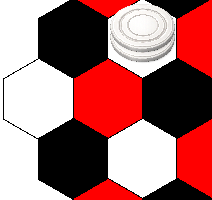
\includegraphics[scale=0.5]{game_rules/images/capture_after.png}
            \caption{After capturing, the black piece is removed}
            \label{fig:capture_after}
        \end{figure}
        \item The \textbf{power} of the attacking stack is strictly higher than the power of the defending stack, but not sufficiently high to be a \textbf{capture}: in this case, the opponent's pieces on the destination tile are not removed from the game, but the attacking player gains the control of the defending stack. This move is called an \textbf{imprisonment}. As an example, consider Figure~\ref{fig:imprisonment_before} and Figure~\ref{fig:imprisonment_after}.
        \begin{figure}[h]
            \centering
            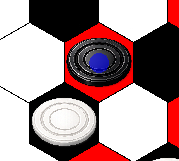
\includegraphics[scale=0.5]{game_rules/images/imprisonment_before.png}
            \caption{Before imprisonment, the attacker (black) has power 3 * 1 = 3 and the defender (white) has power 1 * 2 = 2, so it's an imprisonment}
            \label{fig:imprisonment_before}
        \end{figure}
        \begin{figure}[h]
            \centering
            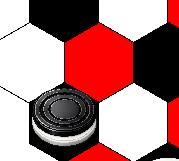
\includegraphics[scale=0.5]{game_rules/images/imprisonment_after.png}
            \caption{After imprisonment, black now controls the defender's tile}
            \label{fig:imprisonment_after}
        \end{figure}
        \item The \textbf{power} of the attacking stack is lower than or equal to the power of the defending stack: in this case, the move isn't allowed.
    \end{enumerate}
    Note: when a "scenario 3" type of move (i.e. the destination tile is controlled by your opponent) is possible to a player, they is forced to make it. If multiple "scenario 3" moves are possible, the player can choose the one they want to make.
\end{enumerate}

\section{Game ending and winner of the game}

A game ends when any player can't make any move. If this happens to a player, the other player wins the game. As an example, consider Figure~\ref{fig:black_win}

\begin{figure}[h]
    \centering
    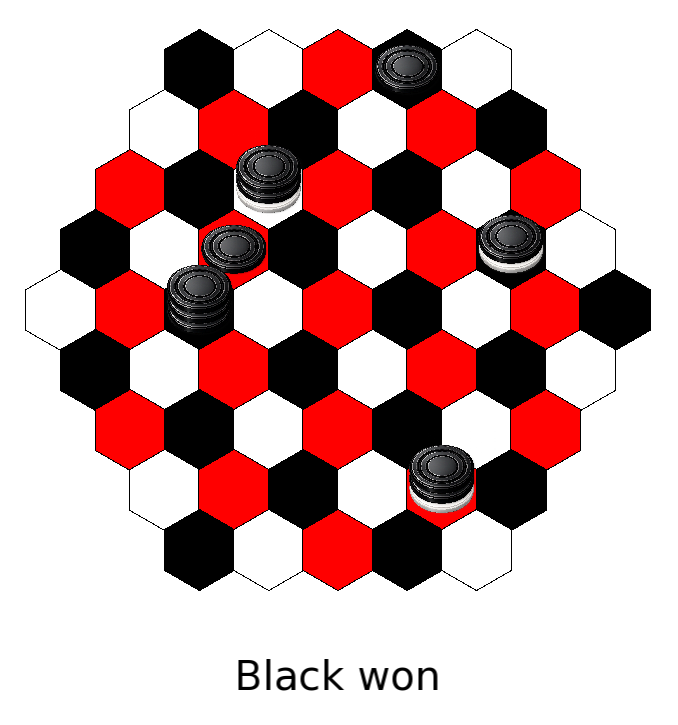
\includegraphics[scale=0.5]{game_rules/images/black_win.png}
    \caption{Example of a finished game won by black. White has no moves.}
    \label{fig:black_win}
\end{figure}

\subsection{Additional rule}
\label{sec:rule_modification}

As explained in the introduction of this chapter, in the patent for the game there are no rules regarding how long a game can last. Therefore, because it's theoretically possible to get to positions where the best strategy for both players is to avoid the opponent's pieces, it's important to add a rule specifying that if no stack was captured in the last 100 turns (each player must play 50 moves), then the game ends and results in a draw. This would avoid infinite length games.